\chapter*{Lampiran}\label{ch:appendix}

\section*{Bukti Email Persetujuan Penggunaan Data}

\begin{figure}[H]
\centering
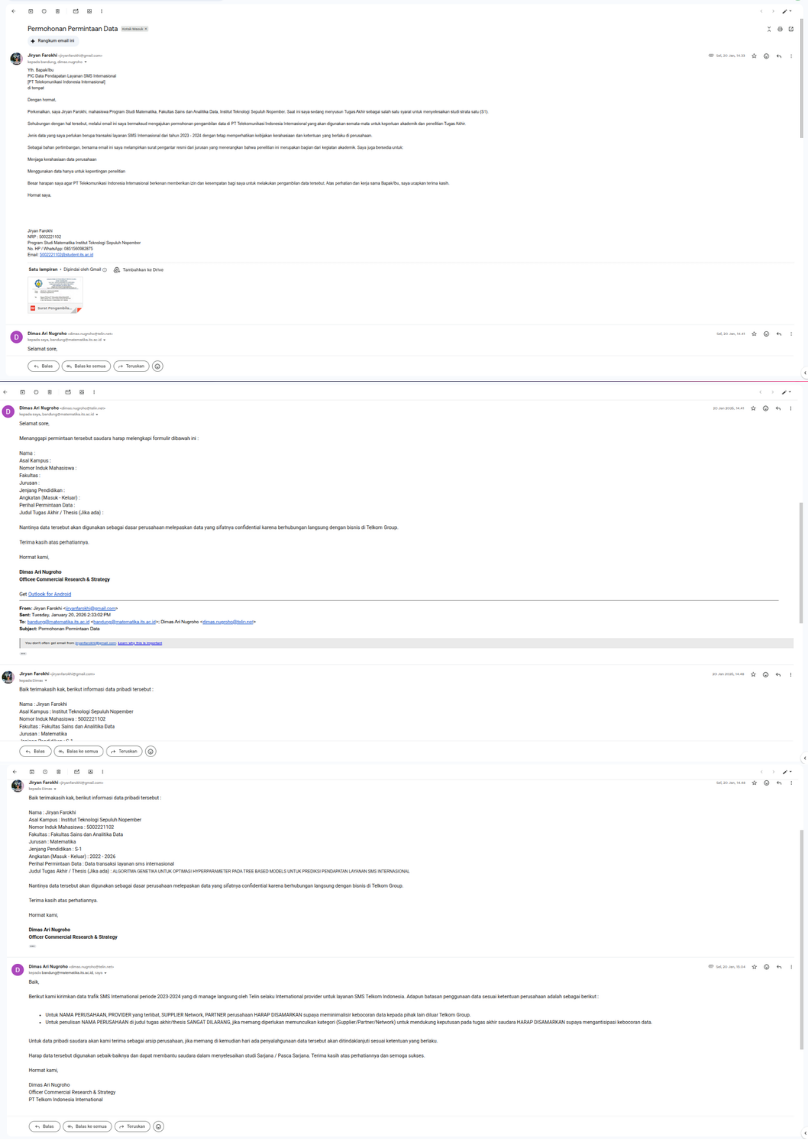
\includegraphics[width=0.7\textwidth]{tugas-akhir/assets/images/buktipersetujuanpenggunaandata.png}
\caption{Bukti Email Persetujuan Penggunaan Data}
\label{fig:plot_forecast}
\end{figure}


\section*{Preview Dataset 50 Data Pertama}\label{ch:lampiran1}

\begin{landscape}
\begin{center}
\captionof{table}{Contoh Data \textit{SMS International} (50 dari 94.335 baris)}
\vspace{12pt}
\begin{adjustbox}{max width=\linewidth}
\renewcommand{\arraystretch}{1.2}
\begin{tabular}{cccccccccccccccrrrrr r}
\toprule
\textbf{Year} & \textbf{Month} & \textbf{Client} & \textbf{ClientConnection} & \textbf{Supplier} & \textbf{SupplierConnection} & \textbf{SupplierConnectionLink} & \textbf{Route} & \textbf{Country} & \textbf{Network} & \textbf{OAProfiledCategory} & \textbf{CostCurrency} & \textbf{PriceCurrency} & \textbf{ProfitCurrency} & \textbf{BaseCurrency} & \textbf{TotalRevenue} & \textbf{TotalCost} & \textbf{TotalSentMessages} & \textbf{TotalDeliveredMessages} & \textbf{TotalUndeliveredMessages} \\
\midrule
2023 & 2  & CLIENT\_031 & CLIENTCONNECTION\_065 & SUPPLIER\_001 & SUPPLIERCONNECTION\_001 & SUPPLIERCONNECTIONLINK\_005 & ROUTE\_041 & Indonesia & NETWORK\_007 & OAPROFILEDCATEGORY\_1391 & USD & USD & USD & USD & 1,401,484 & 1,245,221 & 9,766,437 & 9,079,388 & 157,978 \\
2023 & 5  & CLIENT\_017 & CLIENTCONNECTION\_001 & SUPPLIER\_001 & SUPPLIERCONNECTION\_001 & SUPPLIERCONNECTIONLINK\_005 & ROUTE\_020 & Indonesia & NETWORK\_007 & OAPROFILEDCATEGORY\_1391 & USD & USD & USD & USD & 1,239,724 & 1,215,675 & 5,959,192 & 5,390,105 & 569,087 \\
2023 & 5  & CLIENT\_017 & CLIENTCONNECTION\_001 & SUPPLIER\_001 & SUPPLIERCONNECTION\_001 & SUPPLIERCONNECTIONLINK\_001 & ROUTE\_020 & Indonesia & NETWORK\_007 & OAPROFILEDCATEGORY\_1391 & USD & USD & USD & USD & 1,236,721 & 1,212,211 & 5,942,211 & 5,377,049 & 565,162 \\
2023 & 6  & CLIENT\_017 & CLIENTCONNECTION\_001 & SUPPLIER\_001 & SUPPLIERCONNECTION\_001 & SUPPLIERCONNECTIONLINK\_001 & ROUTE\_020 & Indonesia & NETWORK\_007 & OAPROFILEDCATEGORY\_1391 & USD & USD & USD & USD & 1,193,231 & 1,215,993 & 5,960,748 & 5,187,960 & 772,788 \\
2023 & 6  & CLIENT\_017 & CLIENTCONNECTION\_001 & SUPPLIER\_001 & SUPPLIERCONNECTION\_001 & SUPPLIERCONNECTIONLINK\_005 & ROUTE\_020 & Indonesia & NETWORK\_007 & OAPROFILEDCATEGORY\_1391 & USD & USD & USD & USD & 1,192,948 & 1,215,533 & 5,958,494 & 5,186,730 & 771,764 \\
2023 & 1  & CLIENT\_030 & CLIENTCONNECTION\_071 & SUPPLIER\_001 & SUPPLIERCONNECTION\_001 & SUPPLIERCONNECTIONLINK\_001 & ROUTE\_037 & Indonesia & NETWORK\_007 & OAPROFILEDCATEGORY\_1391 & USD & USD & USD & USD & 1,098,604 & 1,085,830 & 8,516,311 & 7,900,562 & 143,330 \\
2023 & 7  & CLIENT\_017 & CLIENTCONNECTION\_001 & SUPPLIER\_001 & SUPPLIERCONNECTION\_001 & SUPPLIERCONNECTIONLINK\_005 & ROUTE\_020 & Indonesia & NETWORK\_007 & OAPROFILEDCATEGORY\_1391 & USD & USD & USD & USD & 1,065,334 & 1,089,143 & 5,338,934 & 4,631,889 & 707,045 \\
2023 & 7  & CLIENT\_017 & CLIENTCONNECTION\_001 & SUPPLIER\_001 & SUPPLIERCONNECTION\_001 & SUPPLIERCONNECTIONLINK\_001 & ROUTE\_020 & Indonesia & NETWORK\_007 & OAPROFILEDCATEGORY\_1391 & USD & USD & USD & USD & 1,065,215 & 1,089,061 & 5,338,536 & 4,631,369 & 707,167 \\
2023 & 8  & CLIENT\_017 & CLIENTCONNECTION\_001 & SUPPLIER\_001 & SUPPLIERCONNECTION\_001 & SUPPLIERCONNECTIONLINK\_005 & ROUTE\_020 & Indonesia & NETWORK\_007 & OAPROFILEDCATEGORY\_1391 & USD & USD & USD & USD & 1,009,455 & 1,032,313 & 5,060,358 & 4,388,936 & 671,415 \\
2023 & 8  & CLIENT\_017 & CLIENTCONNECTION\_001 & SUPPLIER\_001 & SUPPLIERCONNECTION\_001 & SUPPLIERCONNECTIONLINK\_001 & ROUTE\_020 & Indonesia & NETWORK\_007 & OAPROFILEDCATEGORY\_1391 & USD & USD & USD & USD & 1,008,179 & 1,032,257 & 5,060,085 & 4,383,389 & 671,671 \\
2023 & 9  & CLIENT\_017 & CLIENTCONNECTION\_001 & SUPPLIER\_001 & SUPPLIERCONNECTION\_001 & SUPPLIERCONNECTIONLINK\_005 & ROUTE\_020 & Indonesia & NETWORK\_007 & OAPROFILEDCATEGORY\_1391 & USD & USD & USD & USD & 990,972 & 1,034,318 & 5,070,188 & 4,308,572 & 761,616 \\
2023 & 9  & CLIENT\_017 & CLIENTCONNECTION\_001 & SUPPLIER\_001 & SUPPLIERCONNECTION\_001 & SUPPLIERCONNECTIONLINK\_001 & ROUTE\_020 & Indonesia & NETWORK\_007 & OAPROFILEDCATEGORY\_1391 & USD & USD & USD & USD & 985,980 & 1,029,188 & 5,045,040 & 4,286,868 & 758,172 \\
2023 & 10 & CLIENT\_017 & CLIENTCONNECTION\_001 & SUPPLIER\_001 & SUPPLIERCONNECTION\_001 & SUPPLIERCONNECTIONLINK\_001 & ROUTE\_020 & Indonesia & NETWORK\_007 & OAPROFILEDCATEGORY\_1391 & USD & USD & USD & USD & 973,111 & 1,000,161 & 4,902,752 & 4,230,918 & 671,834 \\
2023 & 10 & CLIENT\_017 & CLIENTCONNECTION\_001 & SUPPLIER\_001 & SUPPLIERCONNECTION\_001 & SUPPLIERCONNECTIONLINK\_005 & ROUTE\_020 & Indonesia & NETWORK\_007 & OAPROFILEDCATEGORY\_1391 & USD & USD & USD & USD & 972,129 & 999,797 & 4,900,966 & 4,226,649 & 674,317 \\
2024 & 1  & CLIENT\_017 & CLIENTCONNECTION\_001 & SUPPLIER\_001 & SUPPLIERCONNECTION\_001 & SUPPLIERCONNECTIONLINK\_001 & ROUTE\_020 & Indonesia & NETWORK\_007 & OAPROFILEDCATEGORY\_1391 & USD & USD & USD & USD & 961,628 & 950,977 & 4,661,653 & 4,180,991 & 480,662 \\
2024 & 1  & CLIENT\_017 & CLIENTCONNECTION\_001 & SUPPLIER\_001 & SUPPLIERCONNECTION\_001 & SUPPLIERCONNECTIONLINK\_005 & ROUTE\_020 & Indonesia & NETWORK\_007 & OAPROFILEDCATEGORY\_1391 & USD & USD & USD & USD & 961,457 & 951,019 & 4,661,860 & 4,180,249 & 481,611 \\
2023 & 3  & CLIENT\_013 & CLIENTCONNECTION\_028 & SUPPLIER\_001 & SUPPLIERCONNECTION\_004 & SUPPLIERCONNECTIONLINK\_006 & ROUTE\_016 & Indonesia & NETWORK\_007 & OAPROFILEDCATEGORY\_1192 & USD & USD & USD & USD & 919,660 & 778,519 & 8,989,829 & 7,417,443 & 937,661 \\
2023 & 3  & CLIENT\_013 & CLIENTCONNECTION\_028 & SUPPLIER\_001 & SUPPLIERCONNECTION\_004 & SUPPLIERCONNECTIONLINK\_002 & ROUTE\_016 & Indonesia & NETWORK\_007 & OAPROFILEDCATEGORY\_1192 & USD & USD & USD & USD & 917,498 & 776,689 & 8,968,699 & 7,402,547 & 932,770 \\
2024 & 3  & CLIENT\_017 & CLIENTCONNECTION\_001 & SUPPLIER\_001 & SUPPLIERCONNECTION\_001 & SUPPLIERCONNECTIONLINK\_005 & ROUTE\_020 & Indonesia & NETWORK\_007 & OAPROFILEDCATEGORY\_1391 & USD & USD & USD & USD & 916,685 & 905,109 & 4,436,810 & 3,985,587 & 451,223 \\
2024 & 3  & CLIENT\_017 & CLIENTCONNECTION\_001 & SUPPLIER\_001 & SUPPLIERCONNECTION\_001 & SUPPLIERCONNECTIONLINK\_001 & ROUTE\_020 & Indonesia & NETWORK\_007 & OAPROFILEDCATEGORY\_1391 & USD & USD & USD & USD & 916,659 & 904,948 & 4,436,022 & 3,985,474 & 450,548 \\
2023 & 12 & CLIENT\_017 & CLIENTCONNECTION\_001 & SUPPLIER\_001 & SUPPLIERCONNECTION\_001 & SUPPLIERCONNECTIONLINK\_005 & ROUTE\_020 & Indonesia & NETWORK\_007 & OAPROFILEDCATEGORY\_1391 & USD & USD & USD & USD & 912,402 & 920,357 & 4,511,554 & 3,966,966 & 544,588 \\
2023 & 12 & CLIENT\_017 & CLIENTCONNECTION\_001 & SUPPLIER\_001 & SUPPLIERCONNECTION\_001 & SUPPLIERCONNECTIONLINK\_001 & ROUTE\_020 & Indonesia & NETWORK\_007 & OAPROFILEDCATEGORY\_1391 & USD & USD & USD & USD & 911,863 & 919,831 & 4,508,976 & 3,964,621 & 544,355 \\
2023 & 4  & CLIENT\_017 & CLIENTCONNECTION\_001 & SUPPLIER\_001 & SUPPLIERCONNECTION\_001 & SUPPLIERCONNECTIONLINK\_001 & ROUTE\_020 & Indonesia & NETWORK\_007 & OAPROFILEDCATEGORY\_1391 & USD & USD & USD & USD & 905,329 & 921,216 & 4,515,767 & 3,936,215 & 579,552 \\
2023 & 4  & CLIENT\_017 & CLIENTCONNECTION\_001 & SUPPLIER\_001 & SUPPLIERCONNECTION\_001 & SUPPLIERCONNECTIONLINK\_005 & ROUTE\_020 & Indonesia & NETWORK\_007 & OAPROFILEDCATEGORY\_1391 & USD & USD & USD & USD & 904,915 & 921,114 & 4,515,266 & 3,934,414 & 580,852 \\
2023 & 4  & CLIENT\_013 & CLIENTCONNECTION\_028 & SUPPLIER\_001 & SUPPLIERCONNECTION\_004 & SUPPLIERCONNECTIONLINK\_002 & ROUTE\_016 & Indonesia & NETWORK\_007 & OAPROFILEDCATEGORY\_1192 & USD & USD & USD & USD & 892,816 & 755,795 & 8,727,427 & 7,091,224 & 986,710 \\
2023 & 4  & CLIENT\_013 & CLIENTCONNECTION\_028 & SUPPLIER\_001 & SUPPLIERCONNECTION\_004 & SUPPLIERCONNECTIONLINK\_006 & ROUTE\_016 & Indonesia & NETWORK\_007 & OAPROFILEDCATEGORY\_1192 & USD & USD & USD & USD & 892,773 & 755,759 & 8,727,006 & 7,089,587 & 988,001 \\
2024 & 2  & CLIENT\_017 & CLIENTCONNECTION\_001 & SUPPLIER\_001 & SUPPLIERCONNECTION\_001 & SUPPLIERCONNECTIONLINK\_005 & ROUTE\_020 & Indonesia & NETWORK\_007 & OAPROFILEDCATEGORY\_1391 & USD & USD & USD & USD & 888,989 & 877,699 & 4,302,446 & 3,865,168 & 437,278 \\
2024 & 2  & CLIENT\_017 & CLIENTCONNECTION\_001 & SUPPLIER\_001 & SUPPLIERCONNECTION\_001 & SUPPLIERCONNECTIONLINK\_001 & ROUTE\_020 & Indonesia & NETWORK\_007 & OAPROFILEDCATEGORY\_1391 & USD & USD & USD & USD & 887,783 & 876,306 & 4,295,618 & 3,859,925 & 435,693 \\
2023 & 5  & CLIENT\_013 & CLIENTCONNECTION\_028 & SUPPLIER\_001 & SUPPLIERCONNECTION\_004 & SUPPLIERCONNECTIONLINK\_002 & ROUTE\_016 & Indonesia & NETWORK\_007 & OAPROFILEDCATEGORY\_1192 & USD & USD & USD & USD & 881,111 & 745,886 & 8,613,008 & 7,069,540 & 920,428 \\
2023 & 5  & CLIENT\_013 & CLIENTCONNECTION\_028 & SUPPLIER\_001 & SUPPLIERCONNECTION\_004 & SUPPLIERCONNECTIONLINK\_006 & ROUTE\_016 & Indonesia & NETWORK\_007 & OAPROFILEDCATEGORY\_1192 & USD & USD & USD & USD & 871,363 & 737,635 & 8,517,720 & 6,992,868 & 909,522 \\
2023 & 11 & CLIENT\_017 & CLIENTCONNECTION\_001 & SUPPLIER\_001 & SUPPLIERCONNECTION\_001 & SUPPLIERCONNECTIONLINK\_001 & ROUTE\_020 & Indonesia & NETWORK\_007 & OAPROFILEDCATEGORY\_1391 & USD & USD & USD & USD & 860,531 & 881,575 & 4,321,448 & 3,741,441 & 580,007 \\
2023 & 11 & CLIENT\_017 & CLIENTCONNECTION\_001 & SUPPLIER\_001 & SUPPLIERCONNECTION\_001 & SUPPLIERCONNECTIONLINK\_005 & ROUTE\_020 & Indonesia & NETWORK\_007 & OAPROFILEDCATEGORY\_1391 & USD & USD & USD & USD & 859,805 & 880,930 & 4,318,286 & 3,738,284 & 580,002 \\
2023 & 3  & CLIENT\_013 & CLIENTCONNECTION\_028 & SUPPLIER\_001 & SUPPLIERCONNECTION\_004 & SUPPLIERCONNECTIONLINK\_006 & ROUTE\_016 & Indonesia & NETWORK\_007 & OAPROFILEDCATEGORY\_3758 & USD & USD & USD & USD & 831,216 & 703,649 & 8,125,275 & 6,727,354 & 1,031,719 \\
2023 & 3  & CLIENT\_013 & CLIENTCONNECTION\_028 & SUPPLIER\_001 & SUPPLIERCONNECTION\_004 & SUPPLIERCONNECTIONLINK\_002 & ROUTE\_016 & Indonesia & NETWORK\_007 & OAPROFILEDCATEGORY\_3758 & USD & USD & USD & USD & 829,778 & 702,432 & 8,111,224 & 6,716,929 & 1,028,377 \\
2023 & 1  & CLIENT\_013 & CLIENTCONNECTION\_028 & SUPPLIER\_001 & SUPPLIERCONNECTION\_004 & SUPPLIERCONNECTIONLINK\_002 & ROUTE\_016 & Indonesia & NETWORK\_007 & OAPROFILEDCATEGORY\_1192 & USD & USD & USD & USD & 810,829 & 686,391 & 7,925,994 & 6,549,499 & 819,832 \\
2023 & 1  & CLIENT\_013 & CLIENTCONNECTION\_028 & SUPPLIER\_001 & SUPPLIERCONNECTION\_004 & SUPPLIERCONNECTIONLINK\_006 & ROUTE\_016 & Indonesia & NETWORK\_007 & OAPROFILEDCATEGORY\_1192 & USD & USD & USD & USD & 810,779 & 686,348 & 7,925,501 & 6,548,783 & 820,443 \\
2023 & 6  & CLIENT\_013 & CLIENTCONNECTION\_028 & SUPPLIER\_001 & SUPPLIERCONNECTION\_004 & SUPPLIERCONNECTIONLINK\_006 & ROUTE\_016 & Indonesia & NETWORK\_007 & OAPROFILEDCATEGORY\_1192 & USD & USD & USD & USD & 809,847 & 685,559 & 7,916,391 & 6,536,815 & 830,352 \\
2023 & 6  & CLIENT\_013 & CLIENTCONNECTION\_028 & SUPPLIER\_001 & SUPPLIERCONNECTION\_004 & SUPPLIERCONNECTIONLINK\_002 & ROUTE\_016 & Indonesia & NETWORK\_007 & OAPROFILEDCATEGORY\_1192 & USD & USD & USD & USD & 805,776 & 682,113 & 7,876,599 & 6,501,031 & 827,723 \\
2024 & 3  & CLIENT\_013 & CLIENTCONNECTION\_028 & SUPPLIER\_001 & SUPPLIERCONNECTION\_004 & SUPPLIERCONNECTIONLINK\_002 & ROUTE\_016 & Indonesia & NETWORK\_007 & OAPROFILEDCATEGORY\_3758 & USD & USD & USD & USD & 792,204 & 670,625 & 7,743,932 & 6,437,084 & 917,715 \\
2024 & 3  & CLIENT\_013 & CLIENTCONNECTION\_028 & SUPPLIER\_001 & SUPPLIERCONNECTION\_004 & SUPPLIERCONNECTIONLINK\_006 & ROUTE\_016 & Indonesia & NETWORK\_007 & OAPROFILEDCATEGORY\_3758 & USD & USD & USD & USD & 791,645 & 670,152 & 7,738,470 & 6,432,588 & 917,044 \\
2023 & 3  & CLIENT\_017 & CLIENTCONNECTION\_001 & SUPPLIER\_001 & SUPPLIERCONNECTION\_001 & SUPPLIERCONNECTIONLINK\_001 & ROUTE\_020 & Indonesia & NETWORK\_007 & OAPROFILEDCATEGORY\_1391 & USD & USD & USD & USD & 774,855 & 830,830 & 4,072,695 & 3,443,902 & 628,793 \\
2023 & 2  & CLIENT\_013 & CLIENTCONNECTION\_028 & SUPPLIER\_001 & SUPPLIERCONNECTION\_004 & SUPPLIERCONNECTIONLINK\_006 & ROUTE\_016 & Indonesia & NETWORK\_007 & OAPROFILEDCATEGORY\_1192 & USD & USD & USD & USD & 755,581 & 639,622 & 7,385,932 & 6,143,402 & 738,106 \\
2023 & 2  & CLIENT\_013 & CLIENTCONNECTION\_028 & SUPPLIER\_001 & SUPPLIERCONNECTION\_004 & SUPPLIERCONNECTIONLINK\_002 & ROUTE\_016 & Indonesia & NETWORK\_007 & OAPROFILEDCATEGORY\_1192 & USD & USD & USD & USD & 755,534 & 639,582 & 7,385,472 & 6,143,525 & 738,090 \\
2023 & 1  & CLIENT\_013 & CLIENTCONNECTION\_028 & SUPPLIER\_001 & SUPPLIERCONNECTION\_004 & SUPPLIERCONNECTIONLINK\_006 & ROUTE\_016 & Indonesia & NETWORK\_007 & OAPROFILEDCATEGORY\_3758 & USD & USD & USD & USD & 753,265 & 637,661 & 7,363,296 & 6,180,515 & 867,061 \\
2023 & 1  & CLIENT\_013 & CLIENTCONNECTION\_028 & SUPPLIER\_001 & SUPPLIERCONNECTION\_004 & SUPPLIERCONNECTIONLINK\_002 & ROUTE\_016 & Indonesia & NETWORK\_007 & OAPROFILEDCATEGORY\_3758 & USD & USD & USD & USD & 752,645 & 637,136 & 7,357,229 & 6,174,895 & 866,668 \\
2023 & 3  & CLIENT\_017 & CLIENTCONNECTION\_001 & SUPPLIER\_001 & SUPPLIERCONNECTION\_001 & SUPPLIERCONNECTIONLINK\_005 & ROUTE\_020 & Indonesia & NETWORK\_007 & OAPROFILEDCATEGORY\_1391 & USD & USD & USD & USD & 750,501 & 805,851 & 3,950,251 & 3,338,391 & 611,860 \\
2023 & 7  & CLIENT\_013 & CLIENTCONNECTION\_028 & SUPPLIER\_001 & SUPPLIERCONNECTION\_004 & SUPPLIERCONNECTIONLINK\_006 & ROUTE\_016 & Indonesia & NETWORK\_007 & OAPROFILEDCATEGORY\_1192 & USD & USD & USD & USD & 740,140 & 626,550 & 7,234,994 & 6,016,647 & 760,333 \\
2023 & 7  & CLIENT\_013 & CLIENTCONNECTION\_028 & SUPPLIER\_001 & SUPPLIERCONNECTION\_004 & SUPPLIERCONNECTIONLINK\_002 & ROUTE\_016 & Indonesia & NETWORK\_007 & OAPROFILEDCATEGORY\_1192 & USD & USD & USD & USD & 737,533 & 624,344 & 7,209,515 & 5,996,191 & 756,719 \\
2023 & 4  & CLIENT\_013 & CLIENTCONNECTION\_028 & SUPPLIER\_001 & SUPPLIERCONNECTION\_004 & SUPPLIERCONNECTIONLINK\_006 & ROUTE\_016 & Indonesia & NETWORK\_007 & OAPROFILEDCATEGORY\_3758 & USD & USD & USD & USD & 722,776 & 611,852 & 7,065,262 & 5,756,780 & 957,487 \\
2023 & 4  & CLIENT\_013 & CLIENTCONNECTION\_028 & SUPPLIER\_001 & SUPPLIERCONNECTION\_004 & SUPPLIERCONNECTIONLINK\_002 & ROUTE\_016 & Indonesia & NETWORK\_007 & OAPROFILEDCATEGORY\_3758 & USD & USD & USD & USD & 722,650 & 611,745 & 7,064,031 & 5,754,745 & 958,143 \\
\bottomrule
\end{tabular}
\end{adjustbox}

\vspace{4pt}
{\small\textit{Catatan: Nama klien, supplier, dan koneksi telah disamarkan (\textit{masked}) untuk menjaga kerahasiaan data.}}
\end{center}
\end{landscape}

% ============================================================
% lampiran_kode.tex
% File ini berisi KONTEN LAMPIRAN saja (tanpa preamble).
%
% CARA PAKAI:
%   Di bab Lampiran dokumen utama:
%       \section{Kode Program}
%       \input{lampiran_kode}
%
%   Pastikan preamble dokumen utama sudah menyertakan
%   definisi dari lampiran_setup.tex (lihat file tersebut).
% ============================================================

\section*{Kode Program}

\begin{lstlisting}[style=pycode,caption={Import pustaka dan load dataset}]
import pandas as pd
import numpy as np
import matplotlib.pyplot as plt
from pathlib import Path

df = pd.read_csv("data/SMS International.csv")
df.info()
\end{lstlisting}

\begin{lstlisting}[style=pycode,caption={Normalisasi kolom Network}]
# Normalisasi nilai kategorikal sebelum masking
if 'Network' not in df.columns:
    raise ValueError("Kolom 'Network' tidak ditemukan di dataframe.")

# Simpan snapshot sebelum cleaning untuk verifikasi
network_before = df['Network'].astype(str).value_counts(dropna=False)

# Rapikan spasi dan normalisasi typo umum
df['Network'] = df['Network'].astype(str).str.strip()
df['Network'] = df['Network'].replace({
    r'(?i)^telkomcel$': 'Telkomsel',
    r'(?i)^telkomsel$': 'Telkomsel'
}, regex=True)

network_after = df['Network'].astype(str).value_counts(dropna=False)

print("=== Sebelum cleaning (Network) ===")
print(
    network_before.loc[
        [idx for idx in network_before.index if 'telkom' in idx.lower()]
    ] if any('telkom' in idx.lower() for idx in network_before.index)
    else 'Tidak ada nilai Telkom* sebelum cleaning'
)

print("\n=== Sesudah cleaning (Network) ===")
print(
    network_after.loc[
        [idx for idx in network_after.index if 'telkom' in idx.lower()]
    ] if any('telkom' in idx.lower() for idx in network_after.index)
    else 'Tidak ada nilai Telkom* sesudah cleaning'
)
\end{lstlisting}

\begin{lstlisting}[style=pycode,caption={Identifikasi dan masking kolom sensitif}]
# Identifikasi kolom sensitif berdasarkan nama kolom (case-insensitive)
sensitive_keywords = [
    "client", "company", "provider", "supplier",
    "partner", "network", "route", "connection", "oaprofiledcategory"
]

sensitive_columns = [
    col for col in df.columns
    if any(keyword in col.lower() for keyword in sensitive_keywords)
]

def mask_column(series, label):
    """Masking deterministik: nilai unik -> token anonim per kolom."""
    clean_values = sorted(series.dropna().astype(str).unique())
    mapping = {
        value: f"{label}_{idx:03d}"
        for idx, value in enumerate(clean_values, start=1)
    }
    masked = series.astype(str).map(mapping)
    masked = masked.where(series.notna(), np.nan)
    return masked, mapping

masking_maps = {}

for col in sensitive_columns:
    masked_series, mapping = mask_column(df[col], col.upper())
    df[col] = masked_series
    masking_maps[col] = mapping

print("Kolom yang dimasking:", sensitive_columns)
print("Contoh data setelah masking:")
display(df.head(3))
\end{lstlisting}

\begin{lstlisting}[style=pycode,caption={Pembersihan kolom tidak diperlukan}]
df = df.drop(columns=['Unnamed: 21', 'Unnamed: 22'], errors='ignore')
df.to_csv("data/SMS_International_masked.csv", index=False)
\end{lstlisting}

\begin{lstlisting}[style=pycode,caption={Agregasi temporal dan perhitungan MoM growth}]
# Pastikan kolom numerik temporal siap dihitung
temporal_cols = ['TotalRevenue', 'TotalCost', 'TotalSentMessages']
for col in temporal_cols:
    df_terurut[col] = pd.to_numeric(
        df_terurut[col].astype(str)
            .str.replace(',', '', regex=False)
            .str.replace(' ', '', regex=False),
        errors='coerce'
    )

# Agregasi bulanan
temporal_summary = (
    df_terurut
    .groupby(['Year', 'Month'], as_index=False)[temporal_cols]
    .sum()
    .sort_values(['Year', 'Month'])
    .reset_index(drop=True)
)

# Hitung pertumbuhan month-to-month (%)
for col in temporal_cols:
    temporal_summary[f'{col}_MoM_pct'] = (
        temporal_summary[col].pct_change() * 100
    )

print('Ringkasan temporal (5 baris pertama):')
display(temporal_summary.head())
\end{lstlisting}

\begin{lstlisting}[style=pycode,caption={Visualisasi tren temporal dan pertumbuhan MoM}]
# Tren individual -- masing-masing figure terpisah
plot_configs = [
    ('TotalRevenue',      'Tren Total Revenue Bulanan',       'tren_revenue.png'),
    ('TotalCost',         'Tren Total Cost Bulanan',          'tren_cost.png'),
    ('TotalSentMessages', 'Tren Total Sent Messages Bulanan', 'tren_sent_messages.png'),
]

for col, title, fname in plot_configs:
    fig, ax = plt.subplots(figsize=(12, 4))
    ax.plot(temporal_summary.index, temporal_summary[col],
            marker='o', linewidth=2)
    ax.set_title(title)
    ax.set_ylabel(col)
    ax.set_xlabel('Periode (urut Year-Month)')
    ax.grid(alpha=0.3)
    plt.tight_layout()
    plt.savefig(fname, dpi=150, bbox_inches='tight')
    plt.show()

# Pertumbuhan MoM Revenue vs Cost
fig, ax = plt.subplots(figsize=(12, 5))
ax.plot(temporal_summary.index,
        temporal_summary['TotalRevenue_MoM_pct'],
        marker='o', label='Revenue MoM %')
ax.plot(temporal_summary.index,
        temporal_summary['TotalCost_MoM_pct'],
        marker='o', label='Cost MoM %')
ax.axhline(0, color='gray', linestyle='--', linewidth=1)
ax.set_title('Pertumbuhan Bulanan Revenue dan Cost (MoM %)')
ax.set_xlabel('Periode (urut Year-Month)')
ax.set_ylabel('Growth (%)')
ax.legend()
ax.grid(alpha=0.3)
plt.tight_layout()
plt.savefig('tren_mom_growth.png', dpi=150, bbox_inches='tight')
plt.show()
\end{lstlisting}

\begin{lstlisting}[style=pycode,caption={Matriks korelasi Pearson dan heatmap}]
import seaborn as sns

# Pilih kolom numerik
numeric_cols = [
    'TotalRevenue', 'TotalCost', 'TotalSentMessages',
    'TotalDeliveredMessages', 'TotalUndeliveredMessages'
]
df_numeric = df_terurut[numeric_cols].copy()

for col in numeric_cols:
    df_numeric[col] = pd.to_numeric(
        df_numeric[col].astype(str).str.replace(',', ''),
        errors='coerce'
    )

# Hitung korelasi Pearson
correlation_matrix = df_numeric.corr(method='pearson')
print("=== Matriks Korelasi Pearson ===")
print(correlation_matrix)

# Visualisasi heatmap
plt.figure(figsize=(10, 8))
sns.heatmap(
    correlation_matrix, annot=True, fmt='.3f',
    cmap='coolwarm', center=0, square=True,
    linewidths=1, cbar_kws={"shrink": 0.8}
)
plt.title('Correlation Matrix (Pearson) - Fitur Numerik',
          fontsize=14, fontweight='bold')
plt.tight_layout()
plt.show()

print("\n=== Korelasi dengan TotalRevenue (Descending) ===")
revenue_corr = correlation_matrix['TotalRevenue'].sort_values(ascending=False)
print(revenue_corr)
\end{lstlisting}

\begin{lstlisting}[style=pycode,caption={Bubble chart top-20 Series\_ID berdasarkan transaksi}]
# Bentuk Series_ID dari 3 fitur kategorikal
series_df = df.copy()
for c in ['Client', 'Supplier', 'Route']:
    series_df[c] = series_df[c].fillna('UNKNOWN').astype(str)
series_df['Series_ID'] = (
    series_df['Client'] + ' | ' +
    series_df['Supplier'] + ' | ' +
    series_df['Route']
)

series_df['MonthPeriod'] = pd.to_datetime(
    dict(year=series_df['Year'],
         month=series_df['Month'], day=1),
    errors='coerce'
)
series_df = series_df.dropna(subset=['MonthPeriod'])

# Agregasi jumlah transaksi per Series_ID per bulan
bubble_data = (
    series_df
    .groupby(['Series_ID', 'MonthPeriod'], as_index=False)
    .size()
    .rename(columns={'size': 'JumlahTransaksi'})
)

# Ambil top-20 series
top_n = 20
top_series = (
    bubble_data.groupby('Series_ID', as_index=False)['JumlahTransaksi']
    .sum()
    .sort_values('JumlahTransaksi', ascending=False)
    .head(top_n)['Series_ID']
)
bubble_plot = bubble_data[bubble_data['Series_ID'].isin(top_series)].copy()

series_order = (
    bubble_plot.groupby('Series_ID')['JumlahTransaksi']
    .sum().sort_values(ascending=False).index.tolist()
)
bubble_plot['x_pos'] = bubble_plot['Series_ID'].map(
    {s: i for i, s in enumerate(series_order)}
)

# Bubble chart
plt.figure(figsize=(16, 9))
sns.scatterplot(
    data=bubble_plot, x='x_pos', y='MonthPeriod',
    size='JumlahTransaksi', hue='JumlahTransaksi',
    sizes=(40, 1800), palette='viridis', alpha=0.75,
    edgecolor='black', linewidth=0.4
)
plt.title(
    'Bubble Chart Series_ID vs Bulan (Ukuran = Banyaknya Transaksi)',
    fontsize=14, fontweight='bold'
)
plt.tight_layout()
plt.show()
\end{lstlisting}

\begin{lstlisting}[style=pycode,caption={Penandaan pola anomali pada data transaksi}]
# Konversi kolom ke numerik
for col in ['TotalRevenue', 'TotalCost', 'TotalProfit']:
    df_terurut[col] = (
        df_terurut[col]
        .astype(str)
        .str.replace(',', '', regex=False)
        .str.replace(' ', '', regex=False)
        .str.replace('-', '', regex=False)
        .str.strip()
    )
    df_terurut[col] = pd.to_numeric(df_terurut[col],
                                    errors='coerce').fillna(0)

# Pola 1: Transaksi gagal (0,0,0) -> hapus
mask_failed = ((df_terurut['TotalRevenue'] == 0) &
               (df_terurut['TotalCost']    == 0) &
               (df_terurut['TotalProfit']  == 0))
count_failed = mask_failed.sum()
df_terurut   = df_terurut[~mask_failed].copy()
print(f'Transaksi gagal dihapus : {count_failed}')
print(f'Sisa data               : {len(df_terurut)}')

# Pola 2: Bonus (rev!=0, cost=0, profit=0)
mask_rev_only = ((df_terurut['TotalRevenue'] != 0) &
                 (df_terurut['TotalCost']    == 0) &
                 (df_terurut['TotalProfit']  == 0))
df_terurut['is_anomaly_rev_only'] = mask_rev_only.astype(int)
print(f'Transaksi bonus         : {mask_rev_only.sum()}')

# Pola 3: Testing (rev=0, cost!=0, profit!=0)
mask_cost_only = ((df_terurut['TotalRevenue'] == 0) &
                  (df_terurut['TotalCost']    != 0) &
                  (df_terurut['TotalProfit']  != 0))
df_terurut['is_anomaly_cost_only'] = mask_cost_only.astype(int)
print(f'Transaksi testing       : {mask_cost_only.sum()}')
\end{lstlisting}

\begin{lstlisting}[style=pycode,caption={Agregasi bulanan per Series\_ID}]
# Perbaiki Series_ID -- masukkan Network
df['Series_ID'] = (df['Client'] + '_' + df['Route'] + '_' +
                   df['SupplierConnection'] + '_' + df['Network'])
print(f"Jumlah Series_ID unik: {df['Series_ID'].nunique()}")

group_cols = ['Series_ID', 'Year', 'Month',
              'Client', 'Route', 'SupplierConnection', 'Network']

# Aggregasi anomali
anom_rev = df.groupby(group_cols).agg(
    total_rows=('TotalRevenue', 'count'),
    anomaly_rev_rows=('is_anomaly_rev_only', 'sum')
).reset_index()
anom_rev['anomaly_revenue_pct'] = np.where(
    anom_rev['total_rows'] > 0,
    anom_rev['anomaly_rev_rows'] / anom_rev['total_rows'], 0
)

agg_dict = {
    'TotalRevenue'          : 'sum',
    'TotalCost'             : 'sum',
    'TotalProfit'           : 'sum',
    'TotalSentMessages'     : 'sum',
    'TotalDeliveredMessages': 'sum',
    'TotalUndeliveredMessages': 'sum',
    'is_anomaly_rev_only'   : 'sum',
    'is_anomaly_cost_only'  : 'sum',
    'OAProfiledCategory'    : 'nunique',
}

monthly = df.groupby(group_cols, as_index=False).agg(agg_dict)
monthly = monthly.rename(columns={'OAProfiledCategory': 'unique_OA_count'})
\end{lstlisting}

\begin{lstlisting}[style=pycode,caption={Pembuatan complete panel (cross join series x bulan)}]
# Cross join: setiap series x setiap bulan
all_series = df[['Series_ID', 'Client', 'Route',
                 'SupplierConnection', 'Network']].drop_duplicates()
all_months = sorted(df[['Year', 'Month']].drop_duplicates().values.tolist())
month_df   = pd.DataFrame(all_months, columns=['Year', 'Month'])
panel      = all_series.merge(month_df, how='cross')
panel      = panel.merge(monthly, on=group_cols, how='left')

# Fill bulan tanpa transaksi dengan 0
fill_zero_cols = [
    'TotalRevenue', 'TotalCost', 'TotalProfit',
    'TotalSentMessages', 'TotalDeliveredMessages',
    'TotalUndeliveredMessages', 'is_anomaly_rev_only',
    'is_anomaly_cost_only', 'unique_OA_count',
    'max_OA_revenue', 'min_OA_revenue'
]
for col in fill_zero_cols:
    if col in panel.columns:
        panel[col] = panel[col].fillna(0)

panel['is_active'] = (panel['TotalRevenue'] > 0).astype(int)
panel['rateCost']      = np.where(panel['TotalDeliveredMessages'] > 0,
    panel['TotalCost'] / panel['TotalDeliveredMessages'], 0)
panel['profit_margin'] = np.where(panel['TotalRevenue'] > 0,
    panel['TotalProfit'] / panel['TotalRevenue'], 0)
panel['delivery_rate'] = np.where(panel['TotalSentMessages'] > 0,
    panel['TotalDeliveredMessages'] / panel['TotalSentMessages'], 0)

panel   = panel.sort_values(['Series_ID', 'Year', 'Month']).reset_index(drop=True)
monthly = panel.copy()
print(f'Complete panel shape : {monthly.shape}')
print(f'Active months        : {monthly["is_active"].sum()}')
print(f'is_active ratio      : {monthly["is_active"].mean()*100:.1f}%')
\end{lstlisting}

\begin{lstlisting}[style=pycode,caption={Lag features, rolling features, dan streak aktif}]
monthly = monthly.sort_values(['Series_ID', 'Year', 'Month']).reset_index(drop=True)

# Lag features
for lag in [1, 2, 3]:
    monthly[f'rev_lag{lag}']    = monthly.groupby('Series_ID')['TotalRevenue'].shift(lag)
    monthly[f'active_lag{lag}'] = monthly.groupby('Series_ID')['is_active'].shift(lag)

# Rolling features (shift(1) agar tidak bocor)
grp_rev = monthly.groupby('Series_ID')['TotalRevenue']
monthly['rolling_mean_3'] = grp_rev.shift(1).rolling(3).mean().reset_index(level=0, drop=True)
monthly['rolling_mean_6'] = grp_rev.shift(1).rolling(6).mean().reset_index(level=0, drop=True)
monthly['rolling_std_3']  = grp_rev.shift(1).rolling(3).std() .reset_index(level=0, drop=True)
monthly['rolling_std_6']  = grp_rev.shift(1).rolling(6).std() .reset_index(level=0, drop=True)

grp_act = monthly.groupby('Series_ID')['is_active']
monthly['pct_active_3m'] = grp_act.shift(1).rolling(3).mean().reset_index(level=0, drop=True)
monthly['pct_active_6m'] = grp_act.shift(1).rolling(6).mean().reset_index(level=0, drop=True)

# Streak aktif berturut-turut
def active_streak(s):
    streak, count = [], 0
    for val in s.shift(1).fillna(0):
        count = count + 1 if val == 1 else 0
        streak.append(count)
    return pd.Series(streak, index=s.index)

monthly['active_streak'] = monthly.groupby(
    'Series_ID', group_keys=False)['is_active'].apply(active_streak)

# Bulan sejak terakhir aktif
def months_since_active(s):
    result, count = [], 0
    for val in s.shift(1).fillna(0):
        count = 0 if val == 1 else count + 1
        result.append(count)
    return pd.Series(result, index=s.index)

monthly['months_since_active'] = monthly.groupby(
    'Series_ID', group_keys=False)['is_active'].apply(months_since_active)

# Siklikalitas bulan
monthly['month_sin'] = np.sin(2 * np.pi * monthly['Month'] / 12)
monthly['month_cos'] = np.cos(2 * np.pi * monthly['Month'] / 12)

# Target: bulan DEPAN
monthly['target_active']  = monthly.groupby('Series_ID')['is_active'].shift(-1)
monthly['target_revenue'] = monthly.groupby('Series_ID')['TotalRevenue'].shift(-1)
monthly = monthly[monthly['target_active'].notna()].reset_index(drop=True)

print(f"Shape setelah feature engineering : {monthly.shape}")
print(f"Baris Stage 1 (semua)             : {len(monthly)}")
print(f"Baris Stage 2 (aktif)             : {int(monthly['target_active'].sum())}")
\end{lstlisting}

\begin{lstlisting}[style=pycode,caption={Definisi daftar fitur Stage 1 dan Stage 2}]
FEATURES_STAGE1 = [
    # Status historis
    'active_lag1', 'active_lag2', 'active_lag3',
    'active_streak', 'months_since_active',
    'pct_active_3m', 'pct_active_6m',
    # Revenue historis
    'rev_lag1', 'rev_lag2', 'rev_lag3',
    'rolling_mean_3', 'rolling_mean_6',
    # Operasional
    'TotalSentMessages', 'TotalDeliveredMessages',
    'delivery_rate', 'unique_OA_count',
    # Anomali
    'anomaly_count', 'anomaly_revenue_pct',
    # Siklikalitas
    'month_sin', 'month_cos',
]

FEATURES_STAGE2 = [
    # Revenue historis
    'rev_lag1', 'rev_lag2', 'rev_lag3',
    'rolling_mean_3', 'rolling_mean_6',
    'rolling_std_3', 'rolling_std_6',
    # Status historis
    'active_lag1', 'active_lag2',
    'active_streak', 'pct_active_3m', 'pct_active_6m',
    # Operasional & margin
    'TotalSentMessages', 'TotalDeliveredMessages',
    'delivery_rate', 'profit_margin', 'rateCost',
    'unique_OA_count', 'max_OA_revenue',
    # Anomali
    'anomaly_count', 'anomaly_revenue_pct',
    # Siklikalitas
    'month_sin', 'month_cos',
]
\end{lstlisting}

\begin{lstlisting}[style=pycode,caption={Time-based split dan pelatihan XGBoost Classifier}]
from sklearn.metrics import (classification_report, roc_auc_score,
                             average_precision_score)
from xgboost import XGBClassifier
import warnings
warnings.filterwarnings('ignore')

# Time-based split
monthly['period'] = monthly['Year'] * 12 + monthly['Month']
cutoff = monthly['period'].quantile(0.80).astype(int)

train = monthly[monthly['period'] <= cutoff].copy()
test  = monthly[monthly['period'] >  cutoff].copy()

print(f"Train : {len(train)} baris | period {train['period'].min()}-{train['period'].max()}")
print(f"Test  : {len(test)} baris  | period {test['period'].min()}-{test['period'].max()}")

X_train_s1 = train[FEATURES_STAGE1]
y_train_s1 = train['target_active'].astype(int)
X_test_s1  = test[FEATURES_STAGE1]
y_test_s1  = test['target_active'].astype(int)

clf = XGBClassifier(
    n_estimators=1000,
    learning_rate=0.3,
    max_depth=6,
    subsample=1.0,
    colsample_bytree=1.0,
    reg_lambda=1.0,
    scale_pos_weight=(y_train_s1 == 0).sum() / (y_train_s1 == 1).sum(),
    random_state=42,
    eval_metric='logloss',
    early_stopping_rounds=50,
    verbosity=0,
)
clf.fit(X_train_s1, y_train_s1,
        eval_set=[(X_test_s1, y_test_s1)],
        verbose=False)

# Evaluasi
y_pred_s1 = clf.predict(X_test_s1)
y_prob_s1 = clf.predict_proba(X_test_s1)[:, 1]

print("\n-- Stage 1: Classification Report --")
print(classification_report(y_test_s1, y_pred_s1,
                             target_names=['Idle', 'Active']))
print(f"ROC-AUC           : {roc_auc_score(y_test_s1, y_prob_s1):.4f}")
print(f"Average Precision : {average_precision_score(y_test_s1, y_prob_s1):.4f}")
\end{lstlisting}

\begin{lstlisting}[style=pycode,caption={Definisi hyperparameter space dan fungsi fitness GA}]
import pygad
from sklearn.ensemble import RandomForestRegressor
from xgboost import XGBRegressor
from sklearn.metrics import mean_absolute_error, mean_squared_error, r2_score

def wmape(actual, pred):
    return np.sum(np.abs(actual - pred)) / np.sum(np.abs(actual))

N_FEATURES = len(FEATURES_STAGE2)

# Hyperparameter space Random Forest
RF_GENE_SPACE = [
    {'low': 50,  'high': 1000},        # n_estimators
    {'low': 1,   'high': 7},           # max_depth
    {'low': 2,   'high': 20},          # min_samples_split
    {'low': 1,   'high': 50},          # min_samples_leaf
    {'low': 1,   'high': N_FEATURES},  # max_features
    {'low': 0.1, 'high': 1.0},         # max_samples
]

def decode_rf(solution):
    return {
        'n_estimators'     : int(round(solution[0])),
        'max_depth'        : int(round(solution[1])),
        'min_samples_split': int(round(solution[2])),
        'min_samples_leaf' : int(round(solution[3])),
        'max_features'     : int(round(solution[4])),
        'max_samples'      : float(np.clip(solution[5], 0.1, 1.0)),
    }

# Hyperparameter space XGBoost
XGB_GENE_SPACE = [
    {'low': 0.001, 'high': 1.0},   # learning_rate
    {'low': 50,    'high': 1000},  # n_estimators
    {'low': 1,     'high': 7},     # max_depth
    {'low': 0.1,   'high': 1.0},   # subsample
    {'low': 0.1,   'high': 1.0},   # colsample_bytree
    {'low': 1,     'high': 3},     # reg_lambda
]

def decode_xgb(solution):
    return {
        'learning_rate'   : float(np.clip(solution[0], 0.001, 1.0)),
        'n_estimators'    : int(round(solution[1])),
        'max_depth'       : int(round(solution[2])),
        'subsample'       : float(np.clip(solution[3], 0.1, 1.0)),
        'colsample_bytree': float(np.clip(solution[4], 0.1, 1.0)),
        'reg_lambda'      : float(np.clip(solution[5], 1, 3)),
    }

# Fitness functions
def fitness_rf(ga_instance, solution, solution_idx):
    params = decode_rf(solution)
    model  = RandomForestRegressor(**params, random_state=42, n_jobs=1)
    model.fit(X_train_s2, y_train_s2)
    return -wmape(y_test_s2, model.predict(X_test_s2))

def fitness_xgb(ga_instance, solution, solution_idx):
    params = decode_xgb(solution)
    model  = XGBRegressor(**params, random_state=42, verbosity=0)
    model.fit(X_train_s2, y_train_s2)
    return -wmape(y_test_s2, model.predict(X_test_s2))
\end{lstlisting}

\begin{lstlisting}[style=pycode,caption={Eksekusi GA untuk Random Forest dan XGBoost}]
def on_generation(ga):
    if ga.generations_completed % 10 == 0:
        print(f"  Gen {ga.generations_completed:>3} | "
              f"Best WMAPE: {-ga.best_solution()[1]:.4f}")

# GA -- Random Forest
ga_rf = pygad.GA(
    num_generations=50, num_parents_mating=4,
    fitness_func=fitness_rf, sol_per_pop=40, num_genes=6,
    gene_space=RF_GENE_SPACE, mutation_percent_genes=20,
    crossover_type='scattered', parent_selection_type='tournament',
    K_tournament=3, keep_elitism=2,
    on_generation=on_generation, random_seed=42,
)
ga_rf.run()
best_sol_rf, best_fit_rf, _ = ga_rf.best_solution()
best_params_rf = decode_rf(best_sol_rf)
print(f"Best params RF : {best_params_rf}")
print(f"Best WMAPE RF  : {-best_fit_rf:.4f} ({-best_fit_rf*100:.2f}%)")

# GA -- XGBoost
ga_xgb = pygad.GA(
    num_generations=50, num_parents_mating=4,
    fitness_func=fitness_xgb, sol_per_pop=40, num_genes=6,
    gene_space=XGB_GENE_SPACE, mutation_percent_genes=20,
    crossover_type='scattered', parent_selection_type='tournament',
    K_tournament=3, keep_elitism=2,
    on_generation=on_generation, random_seed=42,
)
ga_xgb.run()
best_sol_xgb, best_fit_xgb, _ = ga_xgb.best_solution()
best_params_xgb = decode_xgb(best_sol_xgb)
print(f"Best params XGB : {best_params_xgb}")
print(f"Best WMAPE XGB  : {-best_fit_xgb:.4f} ({-best_fit_xgb*100:.2f}%)")
\end{lstlisting}

\begin{lstlisting}[style=pycode,caption={Fungsi evaluasi dan perbandingan 4 model}]
def evaluate(name, model, X_tr, y_tr, X_te, y_te):
    model.fit(X_tr, y_tr)
    pred      = model.predict(X_te)
    mae       = mean_absolute_error(y_te, pred)
    rmse      = np.sqrt(mean_squared_error(y_te, pred))
    r2        = r2_score(y_te, pred)
    wmape_val = wmape(y_te, pred)
    mape      = np.mean(np.abs((y_te - pred) /
                np.where(y_te == 0, 1, y_te))) * 100
    print(f"\n{name}")
    print(f"  MAE   : {mae:>14.2f}")
    print(f"  RMSE  : {rmse:>14.2f}")
    print(f"  R2    : {r2:>14.4f}")
    print(f"  WMAPE : {wmape_val*100:>13.2f}%")
    print(f"  MAPE  : {mape:>13.2f}%")
    return {'Model': name, 'MAE': mae, 'RMSE': rmse,
            'R2': r2, 'WMAPE(%)': wmape_val*100, 'MAPE(%)': mape}

results = []
results.append(evaluate("RF Baseline",
    RandomForestRegressor(random_state=42, n_jobs=-1),
    X_train_s2, y_train_s2, X_test_s2, y_test_s2))
results.append(evaluate("RF + GA",
    RandomForestRegressor(**best_params_rf, random_state=42, n_jobs=-1),
    X_train_s2, y_train_s2, X_test_s2, y_test_s2))
results.append(evaluate("XGBoost Baseline",
    XGBRegressor(random_state=42, verbosity=0),
    X_train_s2, y_train_s2, X_test_s2, y_test_s2))
results.append(evaluate("XGBoost + GA",
    XGBRegressor(**best_params_xgb, random_state=42, verbosity=0),
    X_train_s2, y_train_s2, X_test_s2, y_test_s2))

results_df = pd.DataFrame(results)
print("\n== Tabel Ringkasan ==")
print(results_df.to_string(index=False))
print(f"\nModel terbaik (WMAPE): "
      f"{results_df.loc[results_df['WMAPE(%)'].idxmin(), 'Model']}")
\end{lstlisting}

\begin{lstlisting}[style=pycode,caption={Deteksi overfitting -- perbandingan Train vs Test}]
def evaluate_train_test(name, model, X_tr, y_tr, X_te, y_te):
    model.fit(X_tr, y_tr)
    pred_tr = model.predict(X_tr)
    pred_te = model.predict(X_te)

    def _m(y, pred):
        return (mean_absolute_error(y, pred),
                np.sqrt(mean_squared_error(y, pred)),
                r2_score(y, pred),
                wmape(y, pred) * 100)

    tr, te = _m(y_tr, pred_tr), _m(y_te, pred_te)
    return {
        'Model'      : name,
        'Train MAE'  : tr[0], 'Test MAE'  : te[0],
        'Train RMSE' : tr[1], 'Test RMSE' : te[1],
        'Train R2'   : tr[2], 'Test R2'   : te[2],
        'Train WMAPE': tr[3], 'Test WMAPE': te[3],
    }

models_ov = [
    ('RF Baseline',      RandomForestRegressor(random_state=42, n_jobs=-1)),
    ('RF + GA',          RandomForestRegressor(**best_params_rf, random_state=42, n_jobs=-1)),
    ('XGBoost Baseline', XGBRegressor(random_state=42, verbosity=0)),
    ('XGBoost + GA',     XGBRegressor(**best_params_xgb, random_state=42, verbosity=0)),
]

ov_results = [evaluate_train_test(n, m, X_train_s2, y_train_s2,
                                  X_test_s2, y_test_s2)
              for n, m in models_ov]
ov_df = pd.DataFrame(ov_results).set_index('Model')
print(ov_df.round(4).to_string())
\end{lstlisting}

% \begin{lstlisting}[style=pycode,caption={Helper: membangun fitur untuk satu bulan forecast}]
% import math

% def build_features_for_month(hist_df, static_last, year, month):
%     rev = hist_df['TotalRevenue'].values.astype(float)
%     act = hist_df['is_active'].values.astype(float)
%     n   = len(rev)

%     def lag(arr, k):   return float(arr[-k]) if n >= k else 0.0
%     def rmean(arr, w): return float(np.mean(arr[-w:])) if n >= w else (float(np.mean(arr)) if n > 0 else 0.0)
%     def rstd(arr, w):  return float(np.std(arr[-w:], ddof=0)) if n >= w else 0.0

%     streak = 0
%     for v in reversed(act):
%         if v == 1: streak += 1
%         else: break

%     msa = 0
%     for v in reversed(act):
%         if v == 1: break
%         msa += 1

%     return {
%         'active_lag1': lag(act,1), 'active_lag2': lag(act,2),
%         'active_lag3': lag(act,3),
%         'active_streak': float(streak), 'months_since_active': float(msa),
%         'pct_active_3m': rmean(act,3), 'pct_active_6m': rmean(act,6),
%         'rev_lag1': lag(rev,1), 'rev_lag2': lag(rev,2),
%         'rev_lag3': lag(rev,3),
%         'rolling_mean_3': rmean(rev,3), 'rolling_mean_6': rmean(rev,6),
%         'rolling_std_3' : rstd(rev,3),  'rolling_std_6' : rstd(rev,6),
%         'TotalSentMessages'     : float(static_last.get('TotalSentMessages', 0)),
%         'TotalDeliveredMessages': float(static_last.get('TotalDeliveredMessages', 0)),
%         'delivery_rate'         : float(static_last.get('delivery_rate', 0)),
%         'profit_margin'         : float(static_last.get('profit_margin', 0)),
%         'rateCost'              : float(static_last.get('rateCost', 0)),
%         'unique_OA_count'       : float(static_last.get('unique_OA_count', 0)),
%         'max_OA_revenue'        : float(static_last.get('max_OA_revenue', 0)),
%         'anomaly_count'         : float(static_last.get('anomaly_count', 0)),
%         'anomaly_revenue_pct'   : float(static_last.get('anomaly_revenue_pct', 0)),
%         'month_sin': math.sin(2 * math.pi * month / 12),
%         'month_cos': math.cos(2 * math.pi * month / 12),
%     }
% \end{lstlisting}

% \begin{lstlisting}[style=pycode,caption={Loop forecast iteratif Jan--Mar 2025}]
% FORECAST_MONTHS = [(2025, 1), (2025, 2), (2025, 3)]
% MONTH_NAME = {1:'Jan', 2:'Feb', 3:'Mar', 4:'Apr', 5:'May', 6:'Jun',
%               7:'Jul', 8:'Aug', 9:'Sep', 10:'Oct', 11:'Nov', 12:'Dec'}

% all_series_ids = monthly['Series_ID'].unique()
% forecast_rows  = []

% for (yr, mo) in FORECAST_MONTHS:
%     feat_list   = []
%     series_order = []

%     static_last_map = (panel_rolling.groupby('Series_ID')[STATIC_COLS]
%                        .last().to_dict('index'))

%     for sid in all_series_ids:
%         hist    = panel_rolling[panel_rolling['Series_ID'] == sid].sort_values('period')
%         statics = static_last_map.get(sid, {c: 0.0 for c in STATIC_COLS})
%         feat_list.append(build_features_for_month(hist, statics, yr, mo))
%         series_order.append(sid)

%     feat_df      = pd.DataFrame(feat_list)
%     pred_active  = clf.predict(feat_df[FEATURES_STAGE1].values)
%     pred_prob    = clf.predict_proba(feat_df[FEATURES_STAGE1].values)[:, 1]

%     pred_revenue = np.zeros(len(series_order))
%     active_idx   = np.where(pred_active == 1)[0]
%     if len(active_idx) > 0:
%         X_s2_fut = feat_df.iloc[active_idx][FEATURES_STAGE2].values
%         pred_revenue[active_idx] = np.maximum(0, reg_final.predict(X_s2_fut))

%     for i, sid in enumerate(series_order):
%         forecast_rows.append({
%             'Series_ID'   : sid,
%             'Year'        : yr,
%             'Month'       : mo,
%             'Month_Name'  : MONTH_NAME[mo],
%             'Pred_Active' : int(pred_active[i]),
%             'Prob_Active' : round(float(pred_prob[i]), 4),
%             'Pred_Revenue': round(float(pred_revenue[i]), 2),
%         })

%     # Update rolling panel
%     new_rows = pd.DataFrame([{
%         'Series_ID'   : sid,
%         'Year'        : yr, 'Month': mo,
%         'period'      : yr * 12 + mo,
%         'is_active'   : int(pred_active[i]),
%         'TotalRevenue': float(pred_revenue[i]),
%         **{c: static_last_map.get(sid, {}).get(c, 0.0) for c in STATIC_COLS},
%     } for i, sid in enumerate(series_order)])
%     panel_rolling = pd.concat([panel_rolling, new_rows], ignore_index=True)

%     n_active  = int(pred_active.sum())
%     total_rev = float(pred_revenue.sum())
%     print(f"  {MONTH_NAME[mo]} {yr}  ->  "
%           f"Aktif: {n_active:>4} series  |  "
%           f"Total Revenue: {total_rev:>16,.2f}")

% forecast_df = pd.DataFrame(forecast_rows)
% forecast_df.to_csv('forecast_jan_mar_2025.csv', index=False)
% \end{lstlisting}

% \begin{lstlisting}[style=pycode,caption={Plot 10 sample Series\_ID: historis + forecast}]
% import matplotlib.patches as mpatches
% import matplotlib.lines   as mlines

% MONTH_SH = {1:'Jan',2:'Feb',3:'Mar',4:'Apr',5:'May',6:'Jun',
%             7:'Jul',8:'Aug',9:'Sep',10:'Oct',11:'Nov',12:'Dec'}

% active_in_fc = (forecast_df.groupby('Series_ID')['Pred_Active']
%                 .sum().loc[lambda s: s > 0].index.tolist())
% np.random.seed(42)
% sample_ids = list(np.random.choice(active_in_fc, 10, replace=False))

% fig, axes = plt.subplots(2, 5, figsize=(22, 9))
% axes = axes.flatten()
% N_HIST_SHOW = 12

% for ax, sid in zip(axes, sample_ids):
%     hist = (monthly[monthly['Series_ID'] == sid]
%             .sort_values('period').tail(N_HIST_SHOW))
%     hist_rev    = hist['TotalRevenue'].values.astype(float)
%     hist_labels = [f"{MONTH_SH[int(r.Month)]}-{int(r.Year)%100:02d}"
%                    for r in hist.itertuples()]

%     fc = forecast_df[forecast_df['Series_ID'] == sid].sort_values('Month')
%     fc_rev    = fc['Pred_Revenue'].values.astype(float)
%     fc_active = fc['Pred_Active'].values.astype(int)
%     fc_labels = [f"{MONTH_SH[int(r.Month)]}-25" for r in fc.itertuples()]

%     n_h  = len(hist_labels)
%     x_h  = np.arange(n_h)
%     x_f  = np.arange(n_h, n_h + len(fc_labels))

%     ax.plot(x_h, hist_rev, color='steelblue', linewidth=1.8,
%             marker='o', markersize=3.5, zorder=3)
%     ax.fill_between(x_h, hist_rev, alpha=0.12, color='steelblue')

%     if n_h > 0 and len(x_f) > 0:
%         ax.plot([x_h[-1], x_f[0]], [hist_rev[-1], fc_rev[0]],
%                 color='darkorange', linewidth=1.5,
%                 linestyle='--', alpha=0.6)

%     ax.plot(x_f, fc_rev, color='darkorange', linewidth=2,
%             marker='s', markersize=6, linestyle='--', zorder=4)

%     for xj, rv, act in zip(x_f, fc_rev, fc_active):
%         if act == 0:
%             ax.scatter([xj], [rv], marker='x', color='red',
%                        s=80, linewidths=2, zorder=5)

%     ax.grid(alpha=0.2)

% h1 = mpatches.Patch(color='steelblue',  alpha=0.8, label='Historis (aktual)')
% h2 = mpatches.Patch(color='darkorange', alpha=0.8, label='Forecast Jan-Mar 2025')
% h3 = mlines.Line2D([], [], color='red', marker='x', linestyle='None',
%                    markersize=8, markeredgewidth=2, label='Idle (inactive)')

% fig.legend(handles=[h1, h2, h3], loc='lower center', ncol=3,
%            fontsize=10, bbox_to_anchor=(0.5, -0.01))
% fig.suptitle('Revenue Historis & Forecast Jan-Mar 2025',
%              fontsize=13, fontweight='bold', y=1.01)
% plt.tight_layout(rect=[0, 0.05, 1, 1])
% plt.savefig('forecast_sample_series.png', dpi=150, bbox_inches='tight')
% plt.show()
% \end{lstlisting}